\documentclass[11pt,a4paper]{article}
\usepackage[a4paper,margin=2.4cm]{geometry}
\usepackage{amsmath,amssymb,mathtools}
\usepackage{fontspec}
\usepackage{polyglossia}
\setmainlanguage{english}
\setotherlanguage{russian}
\setmainfont{Liberation Serif}
\setsansfont{Liberation Sans}
\setmonofont{Liberation Mono}
\newfontfamily\cyrillicfont[Ligatures=TeX]{Liberation Serif}
\newfontfamily\cyrillicfontsf[Ligatures=TeX]{Liberation Sans}
\newfontfamily\cyrillicfonttt{Liberation Mono}
\usepackage{booktabs}
\usepackage{enumitem}
\usepackage{graphicx}
\usepackage{float}
\usepackage[hidelinks]{hyperref}

\setlength{\parindent}{0pt}
\setlength{\parskip}{0.5em}
\emergencystretch=1.5em
\setlist{itemsep=0.15em,topsep=0.25em}

\newcommand{\G}{\mathcal{G}_k}
\newcommand{\norm}[1]{\lVert #1\rVert_2}
\newcommand{\E}{\mathbb{E}}
\DeclareMathOperator*{\argmin}{arg\,min}
\DeclareMathOperator{\diag}{diag}
\DeclareMathOperator{\Var}{Var}
\DeclareMathOperator{\sigm}{sigm}
\makeatletter\newcommand{\tabinput}[1]{\@@input #1 }\makeatother

\title{SGD versus Robust SGD under Gradient Uncertainty\\[0.2em]\large Homework mini-project report}
\author{Egor Chulkov, Vladislav Dvornikov, Daria Demeshko}
\date{17 November 2026}

\begin{document}
\maketitle

\noindent\textbf{Team and contributions.}
Egor Chulkov: [contribution].
Vladislav Dvornikov: [contribution].
Daria Demeshko: [contribution].

\section*{Introduction}

We study Robust SGD (R-SGD). Instead of trusting the mini-batch gradient $g_k$, it takes a step
that is good for every gradient in an ellipsoid $\G=\{g_k+S_k^{1/2}u:\norm u\le\rho\}$ built from
the batch. Section~1 derives the step and its properties. Section~2 describes our implementation and
checks. Section~3 compares SGD and R-SGD on logistic regression and a small two-layer network.
Section~4 explains how we made the comparison fair, and Section~5 discusses the results. All code,
results and the commands to reproduce them are in the project folder (Section~6).

\section{Derivation and interpretation}

Below $S\succ0$, so $S^{1/2}$ and $S^{-1/2}$ exist, are symmetric, and $\sqrt{x^TSx}=\norm{S^{1/2}x}$.
Inside one step we write $g=g_k$, $S=S_k$, $\alpha=\alpha_k$.

\textbf{(a) Inner maximum.} For fixed $x$,
$\max_{\norm u\le\rho}(\mu+S^{1/2}u)^Tx=\mu^Tx+\max_{\norm u\le\rho}u^T(S^{1/2}x)=\mu^Tx+\rho\sqrt{x^TSx}$
by Cauchy--Schwarz. For $x\ne0$ the maximum is attained at
\begin{equation*}
u^\star=\rho\,\frac{S^{1/2}x}{\norm{S^{1/2}x}},\qquad c^\star=\mu+\rho\,\frac{Sx}{\sqrt{x^TSx}} .
\end{equation*}
In the local model $f(\theta_k+d)\approx f(\theta_k)+\nabla f(\theta_k)^Td$ the true gradient is unknown.
We only know that it is plausibly in $\G$, so $x$ becomes the step $d$ and $\mu$ becomes $g_k$. A
linear model has no minimum, so the term $\norm d^2/(2\alpha_k)$ keeps the step small.

\textbf{(b) Equivalent problem.} The quadratic term does not depend on $h$, so by (a)
\begin{equation*}
d_k=\argmin_d\varphi(d),\qquad \varphi(d)=g^Td+\rho\sqrt{d^TSd}+\frac{\norm d^2}{2\alpha}. \tag{2}
\end{equation*}
For $\rho=0$, $\varphi$ is a quadratic with gradient $g+d/\alpha$, so $d_k=-\alpha g$, which is SGD.
$\varphi$ is a linear term plus a convex norm term plus a $1/\alpha$-strongly convex quadratic, so it is
strongly convex and coercive. Hence the robust step always exists and is unique, even though $\varphi$
is not differentiable at $d=0$. Multiplying the optimality condition in (d) by $d^T$ also gives
$\norm{d_k}\le\alpha\norm{g_k}$: the robust step is never longer than the SGD step.

\textbf{(c) Zero step.} We show that $d_k=0\iff g^TS^{-1}g\le\rho^2$ (condition (3)).
\begin{itemize}
\item If (3) holds and $d\ne0$, Cauchy--Schwarz gives
$g^Td=(S^{-1/2}g)^T(S^{1/2}d)\ge-\sqrt{g^TS^{-1}g}\sqrt{d^TSd}\ge-\rho\sqrt{d^TSd}$. Hence
$\varphi(d)\ge\norm d^2/(2\alpha)>0=\varphi(0)$, so $d_k=0$.
\item If $d_k=0$, put $d=-tS^{-1}g$ with $t\to0^+$. With $\kappa=\sqrt{g^TS^{-1}g}$, the inequality
$\varphi(d)\ge0$ becomes $-t\kappa^2+\rho t\kappa+O(t^2)\ge0$, so $\kappa\le\rho$.
\end{itemize}
Condition (3) is the same as $0\in\G$. It does \textbf{not} imply $\nabla f(\theta_k)=0$: it only says
that the data cannot rule out a zero gradient. Example: $f=\tfrac12\theta^2$ at $\theta_k=1$, with
$b=2$ observations $3$ and $-1$. Then $g_k=1$, $s_k=4.004$ by formula (4), and
$g_k^2/s_k=0.25\le1=\rho^2$, so R-SGD does not move although $\nabla f=1$.

\textbf{(d) Optimality and the isotropic case.} For $d\ne0$ the function $\varphi$ is differentiable,
and because it is convex the step is optimal exactly when
\begin{equation*}
g_k+\rho\,\frac{S_kd_k}{\sqrt{d_k^TS_kd_k}}+\alpha_k^{-1}d_k=0 .
\end{equation*}
For $S=sI$ this reads $(\alpha^{-1}+\rho\sqrt s/\norm d)\,d=-g$, so $d$ points along $-g$. Writing
$d=-t\,g/\norm g$ gives $t=\alpha(\norm g-\rho\sqrt s)$, which is positive only if
$\norm g>\rho\sqrt s$. Otherwise (3) holds and $d=0$. Together,
$d_k=-\alpha_k(1-\rho\sqrt s/\norm{g_k})_+\,g_k$. For $g_k=0$ we get $\varphi(d)>0$ for all $d\ne0$, so
$d_k=0$.

In the isotropic case only the length changes: $\norm{d}=\alpha(\norm g-\rho\sqrt s)_+$. In the
anisotropic case $d=-\alpha(I+\alpha\rho S/\tau)^{-1}g$ with $\tau=\sqrt{d^TSd}$. Directions with
larger uncertainty are shrunk more, so the direction also turns, from $-g$ towards $-S^{-1}g$ as $\rho$
grows.

\textbf{(e) Conditional descent.} The inequality holds. If $d_k=0$ it is trivial. Otherwise:
\begin{itemize}
\item the descent lemma gives $f(\theta_k+d)\le f(\theta_k)+\nabla f(\theta_k)^Td+\tfrac L2\norm d^2$;
\item since $\nabla f(\theta_k)\in\G$, by (a) we have $\nabla f(\theta_k)^Td\le g^Td+\rho\sqrt{d^TSd}$;
\item multiplying the condition in (d) by $d^T$ gives $g^Td+\rho\sqrt{d^TSd}=-\norm d^2/\alpha$.
\end{itemize}
So $f(\theta_k+d_k)\le f(\theta_k)-(\alpha_k^{-1}-L/2)\norm{d_k}^2$, and $\alpha_k<2/L$ is enough for a
decrease whenever $d_k\ne0$. Containment is the key assumption, and it cannot be checked. If the true
gradient is outside $\G$, $\nabla f^Td$ may be positive. Larger $\rho$ makes containment more likely,
roughly $P(\chi^2_p\le\rho^2)$ if $S_k$ were exact, but gives shorter steps and more zero steps.

\section{Implementation and numerical checks}

\textbf{Gradient observations and $S_k$.} We sample $b$ examples with replacement and compute
per-example gradients in closed form:
\begin{itemize}
\item logistic regression: $u_i=(\sigm(t_i)-y_i)(a_i,1)$;
\item network: back-propagation per example, with $\delta=\sigm(t)-y$, $\partial_{w_2}=\delta h$,
$\partial_{b_1}=\delta\,w_2\odot(1-h^2)$, $\partial_{W_1}=\partial_{b_1}a^T$.
\end{itemize}
Central finite differences agree to $<10^{-8}$ relative error for both models. Noise is added only to
these observations, $v_{k,i}=u_i+\sigma z_{k,i}$. From the same $b$ observations we compute $g_k$ and the
diagonal $S_k$ of formula (4). Since sampling is with replacement, $\E\widehat s_{k,j}=\Var(g_{k,j})$,
the variance of the batch mean.

\textbf{Solver for (2).} For diagonal $S$ the optimality condition gives
$d_j=-\alpha\,\tau g_j/(\tau+\alpha\rho s_j)$ with one unknown $\tau=\sqrt{d^TSd}$, which solves
\begin{equation*}
q(\tau)=\sum_j\frac{\alpha^2s_jg_j^2}{(\tau+\alpha\rho s_j)^2}=1 .
\end{equation*}
\begin{itemize}
\item $q$ decreases from $g^TS^{-1}g/\rho^2$ to $0$, so a root exists exactly when (3) fails. The
zero-step rule is therefore built into the solver: we test (3) first and return $d=0$.
\item We solve $q(\tau)^{-1/2}-1=0$ by Newton's method from $\tau=0$, with a bisection safeguard on
$[0,\alpha\sqrt{g^TSg}]$. This function is concave (by Cauchy--Schwarz), so Newton increases
monotonically to the root, and for $S=sI$ it is exact in one step.
\item Stopping rule: $|q^{-1/2}-1|\le10^{-14}$, or a relative change below $10^{-15}$, or at most 100
iterations.
\item Each iteration costs $O(p)$, which is small next to the $O(bp)$ cost of the gradients. In Python,
however, the fixed overhead makes an R-SGD update 3--4 times slower than an SGD update.
\end{itemize}

\textbf{Checks (part b).} On random test problems and on the noisy quadratic of the Illustration we
got the following.
\begin{center}
\small
\begin{tabular}{@{}lp{0.62\linewidth}@{}}
\toprule
Check & Result \\
\midrule
$\rho=0$ & identical to SGD (1000/1000 problems, and identical trajectories) \\
$\rho\to0$ & $\norm{d+\alpha g}$ goes to 0 linearly in $\rho$ \\
Isotropic formula & max.\ relative error $4.8\cdot10^{-12}$ over 10\,000 problems; Newton takes 1 iteration \\
Zero-step rule & matches (3) in all cases, including $\rho=(1\pm10^{-6})\sqrt{g^TS^{-1}g}$ \\
Condition of 1(d) & residual $\le1.0\cdot10^{-14}$; on average 4.4 Newton iterations (max 9) \\
CVXPY cross-check & our objective is never larger than CVXPY's \\
\bottomrule
\end{tabular}
\end{center}
On the noisy quadratic, R-SGD also took zero steps far from the minimum, at $f$ up to $2.9$ (start
$f=10$). This happens along $\theta_1$, where the gradient is weak and the noise is strong; this is
exactly the situation of 1(c).

\textbf{Batch size (part c).} $\widehat s_{k,j}$ estimates $\Sigma_{jj}/b$, so the uncertainty shrinks
like $1/b$. But the estimate itself is noisy, with relative standard deviation $\sqrt{2/(b-1)}$, so
$b=2$ gives 141\% and $b=8$ gives 53\%. Figure~\ref{fig:batch} confirms both formulas.

Two consequences follow:
\begin{itemize}
\item with small batches the zero-step decisions are close to random;
\item with large batches the robust correction ($\propto\rho/\sqrt b$) disappears and R-SGD behaves like
SGD.
\end{itemize}
Without replacement $\widehat s$ would overestimate the variance by $n/(n-b)$; we checked this
numerically. We therefore used $b=16$.

\begin{figure}[H]
\centering
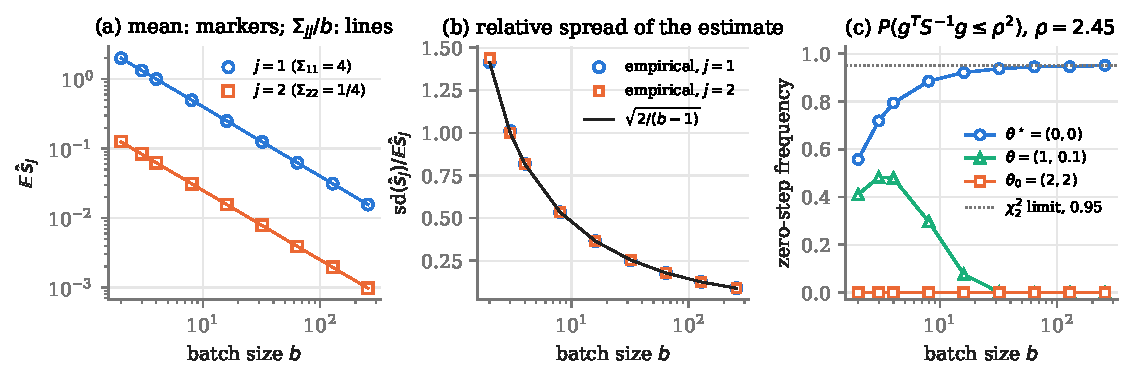
\includegraphics[width=0.92\linewidth]{fig/batch_size.pdf}
\caption{Noisy quadratic, $\sigma=1$, $20\,000$ batches per $b$. (a) $\E\widehat s_j$ follows
$\Sigma_{jj}/b$. (b) Its relative spread follows $\sqrt{2/(b-1)}$. (c) Zero-step frequency for $\rho=2.45$
at three points.}
\label{fig:batch}
\end{figure}

\textbf{Reproducibility (part d).} Everything is in float64. Seeds come from NumPy's
\texttt{SeedSequence}, with separate streams for data, initialisation, batches and noise.
SGD and R-SGD use the same streams (paired runs). The noise touches only the observed gradients; the
objective and all evaluations use clean data. Details are in Section~6.

\section{Required simulations}

\textbf{Setup (both simulations).}
\begin{itemize}
\item Balanced classes, with 400 training, 400 validation and 4000 test points. Inputs are standardised
with training statistics only.
\item Loss: BCE from logits, computed as \texttt{logaddexp(0,t)-y*t}, with no regulariser; we classify
by $t>0$.
\item Budget: $b=16$, $K=500$ updates (logistic) or $K=3000$ (network), and
$\alpha_k=\alpha_0/\sqrt{1+k/50}$ for both methods.
\item Noise: $\sigma=c\,\gamma$ with $c\in\{0,1,4,16\}$, where $\gamma$ is the RMS of per-example
gradients at the start ($0.50$ and $0.215$). The case $c=0$ has no added noise.
\item The radius is written $\rho=r\sqrt p$, because near a minimum $g^TS^{-1}g\approx\chi^2_p$.
\end{itemize}

Settings were tuned on validation data at $c=1$ and then fixed for all noise levels (Section~4):
\begin{itemize}
\item logistic regression: SGD $\alpha_0=0.3$; R-SGD $\alpha_0=1$, $\rho=1.30$;
\item network: SGD $\alpha_0=1$; R-SGD $\alpha_0=10$, $\rho=1.44$.
\end{itemize}
All numbers are means $\pm$ standard deviations over 10 evaluation seeds, each with a new data set.

\subsection{Simulation 1: logistic regression}

The data are $a\mid y\sim\mathcal N((2y-1)(1,1)^T,I)$ and the model is $t=w^Ta+c$ ($p=3$), started from
$\theta_0=0$. The model is correct for this data, so the best possible (Bayes) rule $a_1+a_2>0$ gives
accuracy $0.923$ on our test sets.

\begin{figure}[H]
\centering
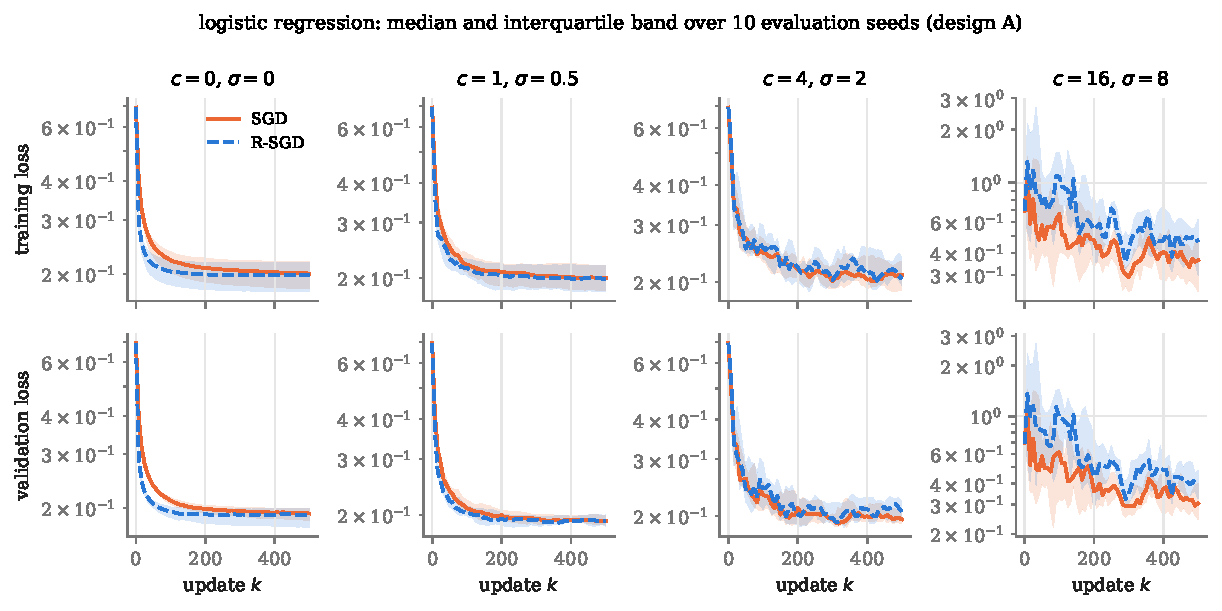
\includegraphics[width=\linewidth]{fig3/logreg_curves.pdf}
\caption{Logistic regression: training (top) and validation (bottom) loss, median and interquartile
band over 10 seeds.}
\label{fig:lr_curves}
\end{figure}

\begin{table}[H]
\centering
\footnotesize
\setlength{\tabcolsep}{3.5pt}
\begin{tabular}{@{}clccccc@{}}
\toprule
$c$ & method & train loss & test loss & accuracy & zero steps & time, ms (µs/update) \\
\midrule
\tabinput{tabs3/tab_lr_main.tex}
\bottomrule
\end{tabular}
\caption{Logistic regression, final results (mean $\pm$ sd over 10 seeds, 8000 gradient evaluations
per run for both methods).}
\label{tab:lr}
\end{table}

\begin{figure}[H]
\centering
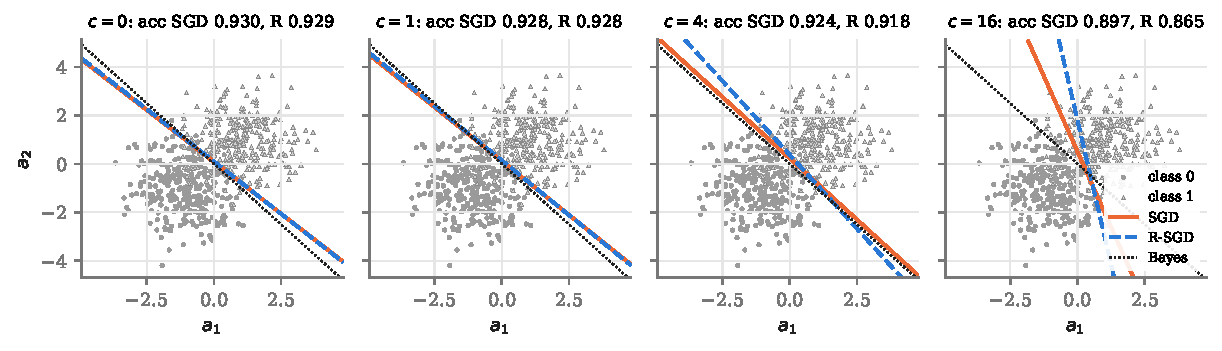
\includegraphics[width=\linewidth]{fig3/logreg_boundaries.pdf}
\caption{Decision boundaries for evaluation seed 0 (dotted: Bayes rule).}
\label{fig:lr_bound}
\end{figure}

Results:
\begin{itemize}
\item Both methods reach the Bayes accuracy for $c\le4$, and the boundaries almost coincide.
\item At low noise R-SGD has a slightly lower loss, by about $0.002$--$0.003$, but the same accuracy.
\item With strong noise ($c=16$) the fixed R-SGD setting is worse: test loss $+0.095$, SGD better in
8/10 seeds.
\item R-SGD takes 18--33\% zero steps but still converges, because $p=3$.
\end{itemize}

\subsection{Simulation 2: two-layer network}

The data are noisy semicircles. The model is $t=w_2^T\tanh(W_1a+b_1)+b_2$ with 8 hidden units
($p=33$). Initialisation: $W_1\sim\mathcal N(0,\tfrac12)$, $w_2\sim\mathcal N(0,\tfrac18)$, zero
biases; both methods start from the same $\theta_0$.

\begin{figure}[H]
\centering
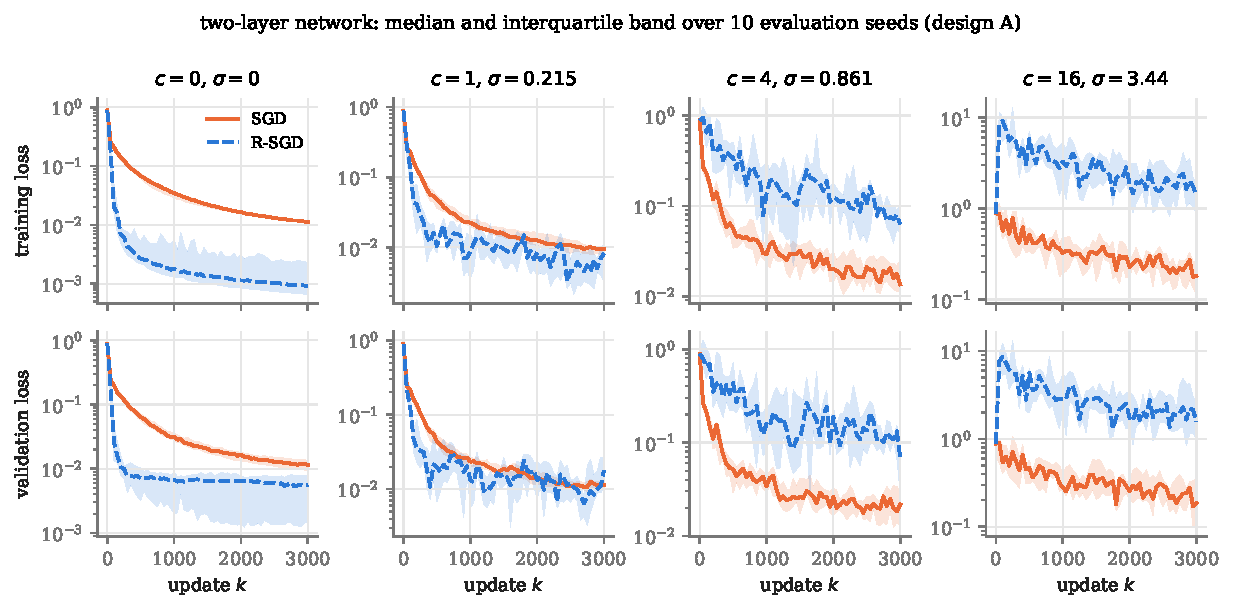
\includegraphics[width=\linewidth]{fig3/mlp_curves.pdf}
\caption{Two-layer network: training (top) and validation (bottom) loss, median and interquartile band
over 10 seeds.}
\label{fig:mlp_curves}
\end{figure}

\begin{table}[H]
\centering
\footnotesize
\setlength{\tabcolsep}{3.5pt}
\begin{tabular}{@{}clccccc@{}}
\toprule
$c$ & method & train loss & test loss & accuracy & zero steps & time, ms (µs/update) \\
\midrule
\tabinput{tabs3/tab_mlp_main.tex}
\bottomrule
\end{tabular}
\caption{Two-layer network, final results (mean $\pm$ sd over 10 seeds, 48\,000 gradient evaluations
per run).}
\label{tab:mlp}
\end{table}

\begin{figure}[H]
\centering
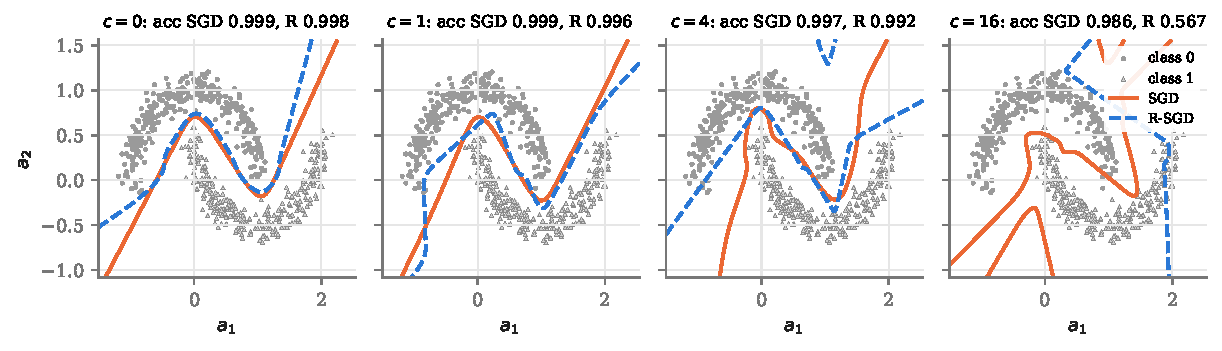
\includegraphics[width=\linewidth]{fig3/mlp_boundaries.pdf}
\caption{Decision boundaries for evaluation seed 0.}
\label{fig:mlp_bound}
\end{figure}

Results:
\begin{itemize}
\item Without noise R-SGD optimises much faster: training loss $0.0019$ vs.\ $0.0110$ (10/10 seeds).
Accuracy is the same, $0.998$.
\item With noise the fixed R-SGD setting is worse. At $c=16$, 8 of 10 runs end above the initial loss
$\log2$, and the boundary in Figure~\ref{fig:mlp_bound} breaks down.
\item No zero steps happen at the chosen $\rho$; the problem is the large step size (Section~5).
\end{itemize}

\subsection{Do optimisation and prediction give the same ranking?}

Not always.
\begin{itemize}
\item At low noise, lower training loss usually also meant lower test loss, but not higher accuracy:
the sign of the training-loss difference predicted the accuracy difference in only 3--5 of 10 seeds.
\item At high noise all rankings agree, with SGD better in 7--10 of 10 seeds.
\end{itemize}

\section{Fair tuning and evaluation}

\textbf{Budgets.} Both methods use the same batch, number of updates and schedule, so they use the same
number of gradient evaluations ($bK$). Runtime is measured over the updates only.

\textbf{Tuning.}
\begin{itemize}
\item Grids: $\alpha_0\in\{0.1,0.3,1,3,10,30\}$ for both methods, and
$r=\rho/\sqrt p\in\{0,0.25,0.5,0.75,1,1.25\}$ for R-SGD; $r=0$ is plain SGD.
\item Criterion: mean validation loss at the end of training, over 3 tuning seeds at $c=1$. Test data
were never used.
\item Search budgets: 18 runs for SGD and 108 for R-SGD.
\item None of the chosen values lies on the edge of its grid (Figure~\ref{fig:tuning}).
\item The surfaces show that larger $\alpha_0$ can be compensated by larger $r$: both control the step
length.
\end{itemize}

\begin{figure}[H]
\centering
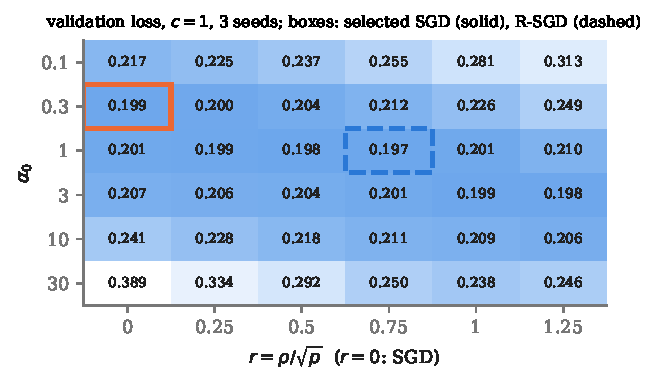
\includegraphics[width=0.48\linewidth]{fig3/logreg_tuning.pdf}\hfill
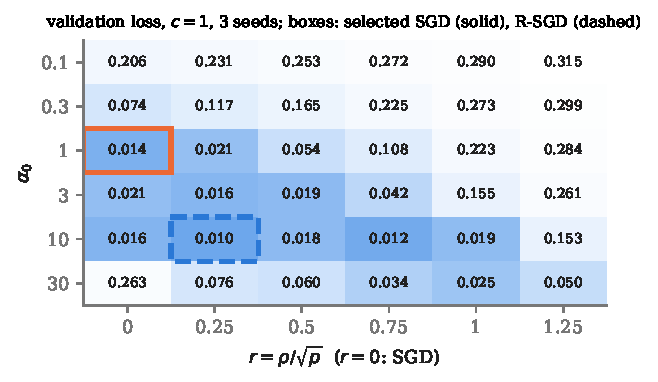
\includegraphics[width=0.48\linewidth]{fig3/mlp_tuning.pdf}
\caption{Validation loss in tuning (left: logistic regression, right: network); boxes mark the chosen
settings.}
\label{fig:tuning}
\end{figure}

\textbf{Seeds and error bars.} We used 10 evaluation seeds with paired runs: the same data,
initialisation, batches and noise for both methods. The error bars are standard deviations over these
seeds. To separate the sources of variability we also ran 10 seeds on one fixed data set. For logistic
regression at low noise most of the spread comes from the data set: the standard deviation of the test
loss is 2--7 times smaller on fixed data. For the network the initialisation matters as much as the data. No run
failed (non-finite loss, or more than 50 times the initial loss).

\textbf{Sensitivity and step length.} We varied $r$ at SGD's $\alpha_0$ (5 seeds,
Figure~\ref{fig:sens}). To check whether a gain is only a shorter step, we also ran SGD with $\alpha_0$
multiplied by R-SGD's mean step ratio $\overline{\norm{d_k}/(\alpha_k\norm{g_k})}$
(Table~\ref{tab:matched}).

\begin{figure}[H]
\centering
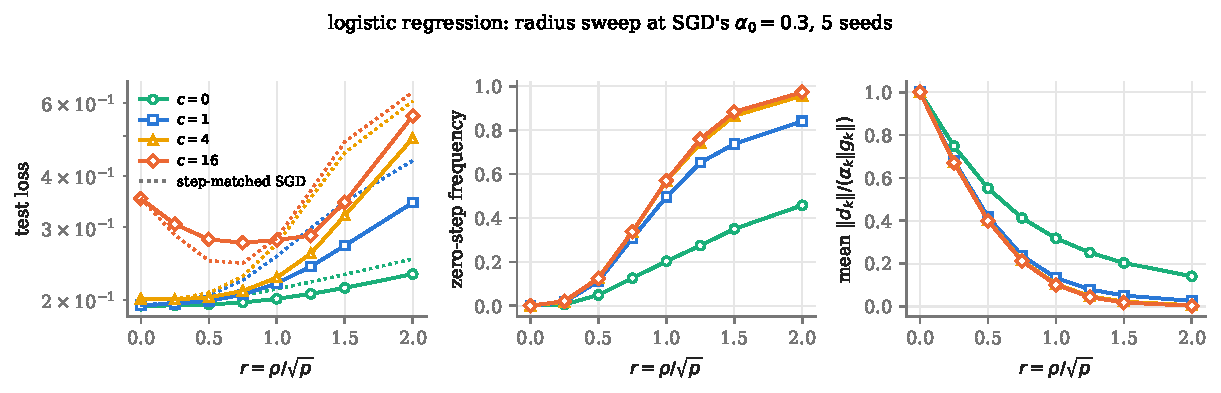
\includegraphics[width=\linewidth]{fig3/logreg_sensitivity.pdf}\\[0.3em]
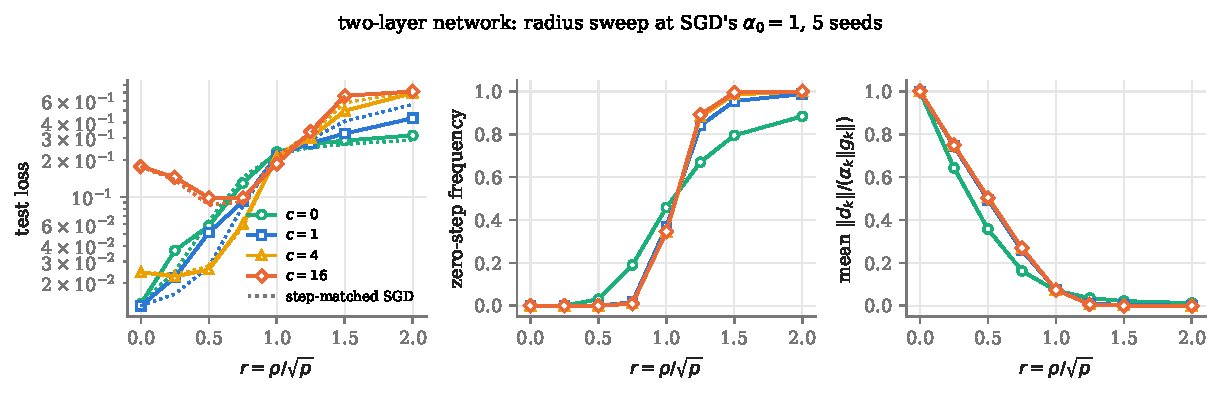
\includegraphics[width=\linewidth]{fig3/mlp_sensitivity.pdf}
\caption{Radius sweep for logistic regression (top) and the network (bottom). Left: test loss of R-SGD
(solid) and of SGD with the same step length (dotted). Middle: zero-step frequency. Right: mean step
ratio.}
\label{fig:sens}
\end{figure}

\begin{table}[H]
\centering
\small
\begin{tabular}{@{}lcccccc@{}}
\toprule
& $c$ & step ratio & R-SGD & SGD, same step & SGD (tuned) & R-SGD better \\
\midrule
Logistic & 0 & 0.30 & 0.1932 & 0.1951 & 0.1951 & 5/10 \\
Logistic & 1 & 0.22 & 0.1949 & 0.1976 & 0.1955 & 9/10 \\
Logistic & 4 & 0.22 & 0.2083 & 0.2029 & 0.2031 & 2/10 \\
Logistic & 16 & 0.22 & 0.4297 & 0.2883 & 0.3343 & 1/10 \\
Network & 0 & 0.59 & 0.0082 & 0.0065 & 0.0133 & 4/10 \\
Network & 1 & 0.74 & 0.0246 & 0.0164 & 0.0126 & 2/10 \\
Network & 4 & 0.74 & 0.1149 & 0.1479 & 0.0246 & 7/10 \\
Network & 16 & 0.74 & 1.9569 & 1.2917 & 0.2241 & 2/10 \\
\bottomrule
\end{tabular}
\caption{Test loss of R-SGD against SGD with the same mean step length (last column: seeds where
R-SGD beats the same-step SGD).}
\label{tab:matched}
\end{table}

In most cases SGD with the same step length is as good as R-SGD or better. The one clear exception is
logistic regression at $c=1$, where R-SGD wins in 9/10 seeds. Radii $r\gtrsim1$ cause many zero steps:
the network gets stuck at accuracy $0.5$--$0.9$.

\section{Critical analysis}

\textbf{(a) When does R-SGD help?}
\begin{itemize}
\item In our experiments only a little, and only for the loss: at low noise in logistic regression,
R-SGD beat both SGD and same-step SGD.
\item There its shrinkage works like an adaptive step-size decay: it is weak at the start, when the
gradients are large and reliable, and strong near the minimum.
\item The big gain of the network at $c=0$ comes from step length: tuning chose a 10 times larger
$\alpha_0$, and SGD with the same effective step does as well.
\item With strong noise R-SGD was worse. When the injected noise dominates, $S_k\approx sI$ and
$\norm{g_k}^2\approx ps$, so by 1(d)
\begin{equation*}
\frac{\norm{d_k}}{\alpha_k\norm{g_k}}\approx1-\frac{\rho}{\sqrt p}.
\end{equation*}
For the network we measured $0.75$, $0.50$, $0.27$ for $r=0.25$, $0.5$, $0.75$.
\item So R-SGD is then just SGD with a shorter step, and it shrinks the largest (noisiest) gradients
the least. It cannot beat a well-tuned SGD there.
\end{itemize}

\textbf{(b) Radius, covariance and learning rate.}
\begin{itemize}
\item $\alpha$ and $\rho$ both control the step length (see the tuning diagonals).
\item The zero-step decision depends only on $\rho$ and $S_k$, not on $\alpha$.
\item $S_k$ scales like $(\text{noise}+\text{sampling variance})/b$, so the same $\rho$ means different
robustness at different $b$ and noise levels.
\item Zero steps happen wherever the gradient is small compared with its noise, not only at a minimum.
On the noisy quadratic this region stretches along $\theta_1$.
\item Under strong noise $g^TS^{-1}g$ looks the same everywhere (about $p(b-1)/(b-3)$), so for
$r\gtrsim1$ zero steps happen almost always. In the network with $r=2$ and $c\ge4$ the parameters never
moved.
\end{itemize}

\textbf{(c) Does lower training loss mean higher accuracy?} No. In the network R-SGD reached
$5.8\times$ lower training loss with the same accuracy. In logistic regression both methods are already
at the Bayes accuracy. Lower cross-entropy here mostly means more confident predictions on points that
are already correct. Only under strong noise, where the boundary itself is damaged, did loss and
accuracy agree.

\textbf{(d) Limitations and next experiment.}
\begin{itemize}
\item We tuned with only 3 seeds at one noise level, and R-SGD had a larger grid. Its chosen network
setting did not repeat its tuning advantage in evaluation (validation loss $0.023$ vs.\ $0.011$ at
$c=1$).
\item The injected noise was isotropic. This is exactly the case where R-SGD reduces to a shorter SGD
step.
\item $S_k$ is diagonal, the problems are small, and our timing is in pure Python.
\end{itemize}
\emph{Next experiment:} add noise only to some parameters, for example the first-layer weights, and
tune both methods separately at each noise level with equal budgets. Then $S_k$ is far from $sI$, and
we can test whether R-SGD's per-coordinate shrinkage beats the best SGD step size.

\section{Reproducibility}

The project folder contains:
\begin{itemize}
\item \texttt{Code/}:
  \begin{itemize}
  \item \texttt{rsgd.py}: estimator, solver and gradient oracles;
  \item \texttt{checks\_section2.py}: Section~2 checks, about 20\,s;
  \item \texttt{sim3\_core.py}, \texttt{sim\_section3.py}: Sections~3--4 (about 3 minutes);
  \item \texttt{make\_tables3.py}: the tables.
  \end{itemize}
\item \texttt{Results/}: all numbers as JSON and NPZ.
\item \texttt{Report/}: this report, its LaTeX source and our more detailed notes.
\end{itemize}
Master seeds are 20261117 (Section~2) and 20261118 (Sections~3--4). We used Python 3.13, NumPy 2.5.3,
SciPy 1.18.1 and Matplotlib 3.11.2.

\begin{thebibliography}{9}
\small
\bibitem{bental} A.~Ben-Tal, L.~El Ghaoui, A.~Nemirovski. \emph{Robust Optimization}. Princeton
University Press, 2009.
\bibitem{bottou} L.~Bottou, F.~E.~Curtis, J.~Nocedal. Optimization methods for large-scale machine
learning. \emph{SIAM Review} 60(2):223--311, 2018.
\bibitem{boyd} S.~Boyd, L.~Vandenberghe. \emph{Convex Optimization}. Cambridge University Press, 2004.
\bibitem{more} J.~J.~Moré, D.~C.~Sorensen. Computing a trust region step. \emph{SIAM J.\ Sci.\ Stat.\
Comput.} 4(3):553--572, 1983.
\bibitem{nocedal} J.~Nocedal, S.~J.~Wright. \emph{Numerical Optimization}, 2nd ed. Springer, 2006.
\end{thebibliography}

\end{document}
